\documentclass[a4paper]{article}

\usepackage{a4wide}
\usepackage{amsmath}
\usepackage{amssymb}
\usepackage{xcolor}
\usepackage{comment}
\usepackage{graphicx}
\usepackage[dutch]{babel}
\usepackage[colorlinks,linkcolor=blue,urlcolor=blue,citecolor=blue]{hyperref}

\title{Elektronisch stemmen \\ \large De ethische discussie over elektronisch stemmen in de digitale samenleving.}
\author{
	Mick van Gelderen \\ 4091566 \and 
	Mick de Lange \\ 1534068 \and
	Salim Salmi \\ 4089715
}

\newcommand{\TODO}[1]{{\color{red}\textbf{TODO: #1}}}

\begin{document}



\maketitle

\hfill \\ \\ \\ \\ \\ \\ \\ \\ \\ \\
\begin{figure}[htp]
	\centering
	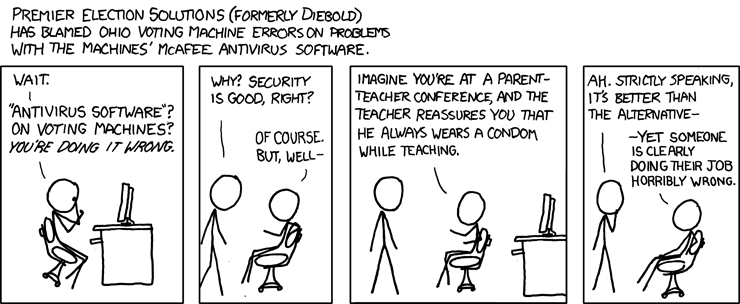
\includegraphics[width=\textwidth]{media/voting_machines.png}
	\label{fig:voting-machines}
	\begin{comment}
		Randall Munroe, (2013), Voting Machines [ONLINE]. Available at: http://imgs.xkcd.com/comics/voting_machines.png [Accessed 15 March 13].
	\end{comment}
\end{figure}

\thispagestyle{empty}
\setcounter{page}{0}
\newpage

\section*{Voorwoord}
Dit artikel is geschreven door 3 studenten Technische Informatica aan de Technische Universiteit Delft voor het vak `informatietechnologie en waarden'.
Het belicht een ethische kwestie van verschillende standpunten aangesterkt met literatuur uit het vakgebied en de filosofie. 

\thispagestyle{empty}

\begingroup
\hypersetup{linkcolor=black}
\tableofcontents
\endgroup

\thispagestyle{empty}
\newpage

\section{Inleiding}

% Inleidend geschiedenis nederland betreft elektronisch stemmen
In de afgelopen jaren is er in Nederland veel te doen geweest rondom elektronisch stemmen.
Zo zijn er een aantal proeven geweest, met verschillende vormen van elektronisch stemmen.
Er zijn naar aanleiding van een aantal problemen actiegroepen opgericht die zich duidelijk uitspraken tegen elektronisch stemmen.
De overheid heeft uiteindelijk verschillende commissies ingesteld die onderzoek hebben gedaan naar de problemen die opspelen bij het inzetten van elektronisch stemmen en naar de benodigdheden om in de toekomst elektronisch stemmen in te voeren.

% Korte belichting moeilijkheden en voordelen
Er spelen binnen dit onderwerp verschillende technische en morele onderwerpen.
Veel genoemd zijn privacy en veiligheid, maar ook de mogelijkheid om bijvoorbeeld gemakkelijker en sneller de stemmen te tellen.
Er zijn op het gebied van elektronisch stemmen dan ook veel problemen, maar ook voordelen.
Op het moment gebruiken we in Nederland weer het papieren stembiljet, maar er zijn ook landen waar wel elektronisch gestemd kan worden.
Wij willen in dit artikel in gaan op de verschillende aspecten en onderzoeken wat deze problemen en voordelen met zich mee brengen.

% Onderzoeksvraag
De precieze onderzoeksvraag is als volgt:
\begin{quote}
\emph{``Zouden we over moeten stappen op elektronisch stemmen?''}
\end{quote}
Deze onderzoeksvraag is het uitgangspunt van dit artikel en we zullen hem naar onze, bij dit onderzoek opgedane, inzichten beantwoorden. 

% Organisatie
In hoofdstuk \ref{text:elektronisch_stemmen} zullen we de gebruikte definitie van elektronisch stemmen bepalen en de verschillende technische en morele aspecten die er spelen belichten.
Aan de hand van deze aspecten zullen we vervolgend de argumenten voor elektronisch stemmen uiteenzetten in hoofdstuk \ref{text:voor}.
Daarna zetten we de argumenten tegen elektronisch stemmen op een rijtje in hoofdstuk \ref{text:tegen}.
Uiteindelijk zullen we aan de hand van deze argumenten onze eigen positie in deze ethische discussie bepalen en toelichten hoe en waarom wij tot deze conclusie zijn gekomen. 
Regeringsinstanties kunnen ons standpunt als advies zien voor de toekomst. 

% Organisatie
Om deze vraag te beantwoorden zullen de verschillende aspecten rondom elektronisch stemmen ter discussie moeten worden gesteld.
Het belichten van deze aspecten en beargumenteren van de pro en con argumenten zal dan uiteindelijk leiden tot een antwoord op deze vraagstelling.

Hierna zullen we eerst verder ingaan op de door ons gebruikte definitie van elektronisch stemmen en de aspecten die daarbij relevant zijn.

\newpage

\section{Elektronisch stemmen}
\label{text:elektronisch_stemmen}
Ten eerste zullen we kort toelichten welke mogelijkheden er zijn voor het toepassen van elektronisch stemmen. 
Vervolgens worden de actoren die een rol spelen worden voorgesteld. 
Daarna worden een aantal technische feiten beschreven zodat het duidelijk is waar elektronisch stemmen over gaat.
Tevens zullen de verschillende morele aspecten omtrent het elektronisch stemmen worden beschreven.
Ten slotte zullen de juridische aspecten die bij het elektronische stemmen komen kijken worden besproken.

\subsection{Mogelijkheden}
Als men het over elektronisch stemmen heeft dan wordt bedoeld het op een over ander manier vastleggen van jouw stem op een digitaal systeem.
Hier is echter nog niet alles mee gezegd, want dit kan op een groot aantal verschillende manieren gebeuren en elk van deze technieken heeft een aantal gevolgen voor de actoren. 

\subsubsection{Stemmen in het stemlokaal}
\label{text:stemlokaal}
De huidige manier van stemmen betreft het invullen van de keuze op een voorgedrukt papieren stembiljet. 
Er zijn een aantal verschillende manieren waarop de stemlokalen gebruik kunnen maken van de digitale techniek.
Hieronder noemen wij er drie. 

% scannen
Het is mogelijk om de stemmen van mensen automatisch vast te leggen door de stembiljetten te scannen.
Op deze manier kan al snel een voorspelling gedaan worden van de uitslagen. 

% elektronisch met papier controle
Een andere mogelijkheid van elektronisch stemmen is het gebruik van een elektronisch stemapparaat met daarnaast een papieren stembiljet voor controle.

% elektronisch met papieren uitdraai
Ten slotte kan ook gebruik gemaakt worden van een stemprinter. 
Hierbij maakt de kiezer elektronisch zijn stem die vervolgens wordt uitgeprint en elektronisch wordt geteld. 
Zo is er een vangnet als de telling niet vertrouwd wordt.

% doel, realistisch
Het voornaamste doel van het implementeren van technologie is hier het vergemakkelijken van de stemmentelling.
Op dit moment worden al naar deze oplossingen gekeken en mee ge{\"e}xperimeerd.

\subsubsection{Stemmen over het internet}
\label{text:internetstemmen}
Tot nu zijn verschillende alternatieven beschreven voor het stemmen in het stemlokaal, waar stemmen priv{\'e} wordt gedaan. 
Maar hoe zit het met stemmen vanuit huis?
Door de opkomst van het internet is de mogelijkheid ontstaan om via het internet te stemmen.

% problemen met stemmen vanuit huis
Bij dit gemak komen ook problemen kijken, zoals veiligheid en fraude. 
Het stemmen over het internet heeft echter een groot fundamenteel probleem waardoor er van wordt afgezien.

% autonomiteit van stemuitbrengende niet gewaarborgd
Er is namelijk geen manier om besloten stemmen te kunnen waarborgen.
Potenti{\"e}le gevolgen kunnen zijn dat bijvoorbeeld druk kan worden uitgeoefend op de kiezer waardoor de kiezer niet meer voor zichzelf stemt.

\subsubsection{Ervaringen van andere landen}
In verschillende landen op de wereld worden vormen van elektronisch stemmen toegepast.
Belangrijke voorbeelden hiervan zullen we hier even kort opsommen.

In Amerika is het mogelijk te stemmen via een stemcomputer met elektronische uitdraai, zoals in \ref{text:stemlokaal} besproken.
Deze oplossing behoudt de mogelijkheid om een handmatige hertelling te doen, om correctheid van de resultaten te garanderen.
Een nadeel zoals dat door veel partijen wordt ervaren is de mogelijke discussie welke telling hogere prioriteit heeft, is dat de papieren telling of de digitale telling? \cite{jacobs2009electronic}

In Estland wordt momenteel een systeem gebruikt waarbij de kiezer vanuit huis met eigen computer kan stemmen. \cite{jacobs2009electronic}
Hiervoor wordt gebruik gemaakt van een \emph{private key}, welke de kiezer heeft op een smartcard.
Een vereiste is dus dat de computer thuis een smartcard kan uitlezen en dat de kiezer deze kaart in zijn bezit heeft en houdt.
Eventuele koppelingen met identiteitsbewijzen met ingebouwde chip zijn denkbaar. 
Zoals besproken in \ref{text:internetstemmen} zijn er mogelijkheden om deze smartcard door te geven en een ander te laten stemmen, of in ergere gevallen kan een gestolen smartcard misbruikt worden om valse stemmen uit te brengen.

In Engeland is enige tijd ge\"{e}xperimenteerd met een digitale telling van de papieren stembiljetten.
Dit is een manier om de verkiezingen alsnog op papier te laten plaatsvinden, maar de telling te automatiseren.
In Nederland is een dergelijke oplossing al snel afgeschreven als mogelijkheid, wegens de zeer grote stembiljetten die hier gebruikt worden. \cite{jacobs2009electronic}
Engeland heeft een politiek systeem dat bestaat uit minder partijen en daardoor ook minder keuzemogelijkheden dan het systeem in Nederland.

\subsection{Betrokken partijen}
De twee meest voor de hand liggende partijen bij verkiezingen zijn natuurlijk de politieke partijen en de burgerlijke kiezers. 
Beiden hebben echter zeer verschillende belangen en standpunten. 
Andere betrokkenen zijn de fabrikanten van de stemapparatuur en software.
Dit zijn partijen die direct te maken hebben met de uitkomst van dit debat.
Er zijn daarnaast ook nog specifieke voor en tegenstanders in dit debat.
Er is een grote groep mensen die hard roepen ``Wij vertrouwen stemcomputers niet", vaak uit angst of gebrek aan kennis en soms uit weloverwogen zin.
Minister Plasterk van Binnenlandse Zaken is een voorstander van elektronisch stemmen en heeft recent een onderzoek ingesteld om te kijken naar de mogelijkheden om het weer in te voeren.

\subsubsection{Kiezers}
De kiezer is de grootste van alle betrokken partijen.
Voor de kiezer is het van belang dat hun stem correct wordt genoteerd en opgeslagen. 
Betrouwbaarheid is voor de burgers dus een belangrijk aspect, immers om verkiezingen te laten werken moeten de stemmen bij de juiste partij terecht komen.
De burger wil tevens niet dat hun privacy op het spel komt te staan, het is niet wenselijk om de uitgebrachte stem openbaar inzichtelijk te hebben.
Het gevolg hiervan kan zijn dat afpersing of omkoping mogelijk wordt, hierover zullen we verder uitweiden in secties \ref{text:moreel} en \ref{text:juridisch}.

\subsubsection{Politieke partijen}
Net zo zeer als burgers hun stem willen waarborgen, willen de politieke partijen dat hun stem niet zomaar door een fout naar een andere partij gaat.
Ook fraude zal voor de politieke partijen een belangrijke rol spelen. 
Een elektronisch systeem waar makkelijk fraude op gepleegd kan worden zal natuurlijk niet geaccepteerd worden.

\subsubsection{Fabrikanten van de stemapparatuur}
De voornaamste leverancier van stemapparatuur in het verleden was een bedrijf genaamd Nedap.
Nedap leverde bijna 90 procent van alle stemcomputers in Nederland.
Toen in 2007 het elektronische stemmen weer werd vervangen door potlood en papier heeft dit voor het bedrijf natuurlijk grote gevolgen gehad.
Daarentegen werd een zekere kwaliteitswaarborg verwacht waar niet aan voldaan was.
Om een actor in dit debat te kunnen blijven zullen de fabrikanten van stemapparatuur en software in moeten kunnen stemmen met de wensen van andere betrokkenen.

\subsubsection{Wij vertrouwen stemcomputers niet}
In 2006 heeft deze groep een website opgericht tegen het gebruik van stemcomputers. 
Zij kwamen toen met het punt dat stemcomputers de verkiezingen voor de burger oncontroleerbaar maken.
Ook vonden zij dat de regelgeving en de techniek van de stemcomputers te kort schoten.

\subsubsection{Minister Plasterk}
De Minister van Binnenlandse Zaken heeft aangegeven dat hij pleit om weer te kijken naar het gebruik van stemcomputers.
Stemmen met het rode potlood is niet meer van deze tijd zegt hij. 
Volgens Plasterk is de techniek al veel vooruitgegaan sinds 2007 toen het gebruik van stemcomputers werd verboden vanwege fraude mogelijkheden.
Plasterk heeft een onderzoek laten instellen om de mogelijkheden tot het opnieuw invoeren van elektronisch stemmen te onderzoeken.
Hierbij is nog geen keuze gemaakt over de vorm waarin dit moet gebeuren, dit moet uit het onderzoek volgen.

\subsection{Morele aspecten}
\label{text:moreel}
Om te bepalen welke morele aspecten er spelen rondom elektronisch stemmen, zullen we eerst moeten kijken naar de geldende normen en waarden rondom het uitbrengen van een stem.
In de huidige vorm van stemmen, met papieren biljetten, zijn een aantal waarden die een belangrijke rol spelen.
Niet al deze waarden hebben altijd een dergelijke rol gehad bij eerdere stemmethoden.
Bij het invoeren van elektronisch stemmen zijn er ook nog andere waarden die een rol gaan spelen, deze komen hier ook aan bod.

\subsubsection{Privacy}
In het huidige kiessysteem is het erg belangrijk dat we onze daadwerkelijke stem voor ons zelf houden.
Ondanks dat iedereen kan vertellen wat hij heeft gestemd, hoeft dit niet de waarheid te zijn en kan iedereen de stem uitbrengen die hij zelf wil.
Deze norm is ontstaan uit de angst voor afpersing of bedreiging, waardoor een kiezer gedwongen kan worden anders te stemmen dan zijn eigen voorkeur.
Omdat dit als een zodanig belangrijk punt wordt gezien is deze norm ook opgenomen in de wetgeving, hierover meer in onderdeel \ref{text:juridisch}: Juridische aspecten.

Overigens speelde privacy niet altijd een dergelijke rol bij het uitbrengen van stemmen.
Zo werd er vroeger ook wel mondeling gestemd, waarbij een persoon fysiek in een publieke ruimte zijn stem uitsprak.
Hierbij was het dus mogelijk om precies te zien wie wat stemde, iets wat in die periode juist als een belangrijke waarde werd gezien.

\subsubsection{Vrijheid}
Om een democratisch systeem te laten werken vinden mensen het van belang dat ieder persoon kan stemmen op de persoon of partij van zijn eigen voorkeur, zonder dat invloeden van buiten af effect hebben op deze keuze.

Deze waarde is enigszins gekoppeld aan de voorgaande waarde: privacy. Er moet namelijk om vrijheid te garanderen geen mogelijkheid zijn tot afpersing of bedreiging.

Ook zijn er natuurlijk andere factoren die invloed kunnen uitoefenen op de stemvoorkeur van een persoon, zoals media en campagnevoering, of bijvoorbeeld groepsdruk.
Deze factoren spelen weliswaar een rol in de keuzevrijheid van het individu, maar zijn even belangrijk bij zowel het huidige papieren stemmen als elektronisch stemmen.
Hier zullen we dan ook niet al te ver op in gaan in dit paper.

\subsubsection{Eerlijkheid en vertrouwen}
Bij verkiezingen zijn eerlijkheid en vertrouwen waarden die dicht bij elkaar liggen en belangrijk zijn.
Hierbij gaat het dan met name over het vertrouwen van de kiezer in de eerlijkheid van het tellen van de stemmen.
Stemmen tellen gebeurt in de huidige papieren vorm met de hand.
De mensen die de telling uitvoeren controleren elkaar om fouten te voorkomen.
Ook zijn de tellingen openbaar toegankelijk voor publiek, om het eerlijk verloop inzichtelijk te maken.
In verkiezingen vinden we het belangrijk dat elke partij of kiespersoon de stemmen krijgt die ook daadwerkelijk zijn uitgebracht op die persoon of partij.

Vertrouwen is heel duidelijk een waarde die in alle vormen van stemmen terug komt.
Zowel in oudere varianten als in elektronisch stemmen speelt dit een rol.
Immers om een juiste verkiezingsuitslag te garanderen is een eerlijke, betrouwbare telling van groot belang.

Door middel van openheid in het proces van stemmen tellen probeert men de eerlijkheid te garanderen.
Het proces moet een open karakter hebben, zodat elke burger begrijpt en ziet hoe de stemmen worden geteld.
Dit begrip en inzicht is voor de burger die zijn stem uitbrengt essentieel om vertrouwen te hebben in het proces.

\subsection{Juridische aspecten}
\label{text:juridisch}
De kieswet ligt vast in het wetboek, deze wet omschrijft de normen die op dit moment gelden rondom verkiezingen \cite{wetboek}.
Deze wetgevingen richten zich er op het stemproces zo goed mogelijk te laten verlopen en een juiste uitslag te garanderen.

Ook worden er in de kieswet veel randzaken vastgelegd, om staatkundig de rechtsgeldigheid van een stem te garanderen.
Dit laatste onderwerp zullen wij hier minder belichten, gezien dit een nauwkeurige omschrijving van het stembiljet betreft, waar bij invoering van elektronisch stemmen de wetgeving uiteraard aanpassingen behoeft.
Overigens dient opgemerkt te worden dat er bij de kortstondige invoering van elektronisch stemmen een artikel aan de wetgeving was toegevoegd die dit mogelijk maakte, welke op dit moment uit de wetgeving is geschrapt.

Wij zullen hier alleen een aantal juridische aspecten toelichten die relevant zijn voor de vraagstelling die in dit paper wordt behandeld.

\subsubsection{Kiesgerechtigden}
Kiesgerechtigden zijn de personen die gerechtigd zijn om bij verkiezingen hun stem uit te brengen \cite{jacobs2009electronic}.
De wet schrijft voor dat deze personen dienen te worden ge\"identificeerd als zodanig bij het uitbrengen van hun stem.
Deze wet voorkomt dat personen die niet gerechtigd zijn om een stem uit te brengen, dit alsnog kunnen doen.
Op deze manier wordt gecontroleerd dat alleen de juiste personen voor de juiste verkiezingen hun stem kunnen uitbrengen.

Hierdoor wordt ook controle gehouden op het aantal keren dat een individu zijn stem kan uitbrengen.
Door de identificatie en het inleveren van de stempas bij het stembureau wordt gecontroleerd dat deze persoon slechts eenmaal kan stemmen.
Wanneer het mogelijk zou worden meerdere malen te stemmen kunnen kwaadwillenden uiteraard de uitslag beïnvloeden.

Het garanderen dat een persoon eenmalig en zelf zijn stem uit brengt is relevant voor elektronisch stemmen. 
Deze twee onderdelen van dit juridische aspect spelen een belangrijke rol in de discussie rond onze vraagstelling over de invoer van elektronisch stemmen.

Wie er precies wel of niet het stemrecht zouden moeten hebben is weer een aparte discussie, hier zullen we in dit artikel dan ook niet verder op in gaan.

\subsubsection{Stemgeheim}
Zoals eerder besproken vinden we het een belangrijke norm dat iemand zijn stemvoorkeur voor zichzelf kan houden.
Deze waarde wordt dusdanig belangrijk gevonden dat het bij wet is vastgelegd \cite{wetboek}.
Deze wet beschermt kiezers voor mogelijke druk van buitenaf om een andere stem uit te brengen dan de persoon zelf zou willen.
De wet verbiedt zelfs de mogelijkheden om bewijs te geven van de stemkeuze.
Dit houdt in dat een persoon wel mag vertellen wat hij gestemd heeft, maar deze persoon behoudt altijd de mogelijkheid hier oneerlijk over te zijn en heeft geen mogelijkheid om te bewijzen of datgene ook juist is.

Deze wetgeving betekent in de praktijk dus dat het niet is toegestaan om samen met iemand anders een stem uit te brengen.
Vandaar ook de verplichting van maximaal {\'e}{\'e}n persoon in een stemhokje.
Het stemgeheim speelt ook een belangrijke rol in de discussie rondom onze vraagstelling, omdat het volgens huidige wetgeving dus niet mogelijk moet zijn om een stem te herleiden naar een persoon.
Bij elektronisch stemmen brengt dit enkele procedurele en technische eisen met zich mee.

\newpage

\section{Waarom niet elektronisch stemmen?}
\label{text:tegen}
In dit hoofdstuk zullen we de belangrijkste argumenten van de tegenstanders van elektronisch stemmen bespreken.
Deze redenen liggen aan de basis van de weerstand tegen elektronisch stemmen.

\subsection{Vertrouwen}
Het ouderwetse stembiljet heeft voor de kiezer een groot persoonlijk voordeel. 
Als het stembiljet wordt ingevuld en gedeponeerd heeft de burger bevestiging dat de zijn stem goed terecht is gekomen. 
Maar hoe zit dat met elektronisch stemmen?
Als men op een machine een keuze in moet vullen, wie zegt dan dat als er op de knop wordt gedrukt er achter de schermen ook echt op die partij gestemd is?
De stemcomputer is voor de kiezer een blackbox, er is geen bevestiging.
De kiezer moet dus maar vertrouwen dat de juiste keuze is gemaakt want zij weten niet wat de machine doet.

In de huidige situatie is het zo dat tijdens de telling van de papieren stembiljetten iedereen mag komen kijken naar de telling.
Zo kan de burger controleren dat de verkiezing eerlijk verloopt.
Deze mogelijkheid is er niet bij het elektronisch stemmen.
De burger heeft geen inzicht op de stemmentelling. 

\subsection{Beveiliging}
Wanneer we praten over veiligheid moeten een aantal aspecten overwogen worden. 
Hoe kan men veiligheid waarborgen? 
Wat zijn de risico's?
Fraude is het eerste wat waar men aan denkt als er over veiligheid wordt gesproken in het debat over elektronisch stemmen.
Dit is tevens ook een van de belangrijkste argumenten tegen het gebruik van stemcomputers tijdens de verkiezingen.
Als er niet gegarandeerd kan worden dat fraude door gebruik te maken van de technologie onmogelijk is, dan zal elektronisch stemmen nooit een mogelijkheid zijn.

\subsection{Privacy}
Voor veel elektronische oplossing moet de stemmer een beetje privacy opgeven.
Om er voor te kunnen zorgen dat iemand niet meerdere keren kan stemmen, zal geregistreerd moeten worden dat hij heeft gestemd. 
Als dit gekoppeld wordt met waar de kiezer voor heeft gekozen ontstaan er privacy problemen.
Er kan namelijk geregistreerd worden wie heeft gestemd op welke partij. 
Dit zijn gegevens die voor veel mensen gevoelig zijn.
Daarnaast is dit in strijd met de huidige wet van het stemgeheim.

\newpage

\section{Waarom wel elektronisch stemmen?}
\label{text:voor}
Er zijn een aantal redenen waarom elektronisch stemmen volgens de voorstander zou moeten worden ingevoerd.
In dit hoofdstuk zullen we de belangrijkste argumenten bespreken, vanuit het oogpunt van de voorstanders.
Hierdoor moet een beeld gecre{\"e}erd worden van de voordelen van elektronisch stemmen.

\subsection{Modernisering}
Een belangrijke reden dat men elektronisch stemmen in wil voeren, is dat stembiljetten niet meer van deze tijd zijn.
Onze wereld wordt steeds meer digitaal, we ontkomen er daarom niet aan om ook naar digitaal stemmen over te stappen.
Hoe kan het dan zo zijn dat we een van de belangrijkste handelingen in onze samenleving op een ouderwetse manier met papier en potlood doen?

Bij het overstappen van gesproken stemmen naar papieren stembiljetten werden ook vele nadelen genoemd, zoals de mogelijkheid om valse stembiljetten te gebruiken of meerdere stembiljetten in te leveren.
Dit soort angstige reacties op nieuwe technieken zouden geen beperking moeten zijn in de ontwikkeling.

\subsection{Effici{\"e}nter}
Een belangrijk voordeel van stemcomputers is dat het tellen van de stemmen altijd honderd procent nauwkeurig gebeurt.
Een computer maakt geen telfouten en een hertelling zal om diezelfde reden ook nooit nodig zijn.
Daarbij geldt ook dat een hertelling niet mogelijk is, een computer zal een tweede keer nooit anders tellen dan de eerste keer, tenzij de invoer veranderd is.
Uiteraard leunt deze uitspraak sterk op de juistheid van de soft- en hardware van een stemcomputer, maar dit is een basiseis voor het invoeren van elektronisch stemmen.

Deze snelle, nauwkeurige, telling levert gelijk ook een ander belangrijk voordeel van elektronisch stemmen.
Het is niet langer nodig om alles met de hand te tellen, waarvoor zeer veel mensen door heel Nederland nodig waren.
Doordat handmatige tellingen en hertelling niet langer nodig zullen zijn hoeven er niet meer zoveel mensen te werken.
Dit levert dus naast een tijdsbesparing ook een enorme geldbesparing op.
De logistiek rondom verkiezingen wordt hierdoor aanzienlijk simpeler en de overhead kosten zullen lager liggen.

Door de snelheid wordt het ook mogelijk om direct een uitslag bekend te maken.
Zodra de stembureaus sluiten is het duidelijk hoeveel stemmen elke partij heeft gekregen.
Hierdoor zal het niet langer nodig zijn om tot diep in de nacht de uitslag af te wachten.

\subsection{Gemakkelijker}
Met stemcomputers wordt stemmen veel gemakkelijker, bij de huidige papieren verkiezingen worden veel biljetten verkeerd ingevuld.
Dit aantal staat gelijk aan een zetel in de tweede kamer.
Bij elektronisch stemmen kan een stem nooit ongeldig zijn, deze is simpelweg juist of blanco.

Daarnaast bieden stemcomputers de mogelijkheden om speciale aanpassingen voor mensen met een visuele handicap te maken.
Hierdoor kunnen deze mensen ook makkelijker hun stem uitbrengen, ze mogen nu immers niet geholpen worden in het stemhokje en de biljetten mogen niet afwijken van de voorschriften.

\newpage

\section{Conclusie}
In dit rapport hebben we de verschillende onderwerpen behandeld die komen kijken bij de invoering van elektronisch stemmen.
Zo hebben we de betrokken partijen behandeld en gezien wat hun belangen zijn en waarom zij eventueel voor of tegen de invoering zijn.
Om te bepalen welke aspecten een rol spelen in de discussie hebben we gekeken welke morele en juridische kwesties spelen rondom verkiezingen in de huidige vorm en in mogelijk elektronische vorm.
Vervolgens zijn de voor- en tegenargumenten uiteengezet, om een beeld te geven van de motivaties voor beide standpunten.

Onze eigen conclusie is dat wij voorstanders zijn van het invoeren van elektronisch stemmen.
In onze huidige samenleving zullen we ook op dit gebied moeten doorgaan met de ontwikkelingen.
De voordelen die wij zien in elektronisch stemmen wegen dan ook zeker op tegen veel bezwaren en sommige bezwaren kunnen worden weggenomen door een goede strategie bij het invoeren.
Het is duidelijk dat er een aantal belangrijke eisen zijn waar aan zal moeten worden voldaan voor dat dit succesvol kan worden ingevoerd.
IN het volgende onderdeel zullen wij uitweiden over deze eisen en onze visie op het succesvol invoeren van elektronisch stemmen.

\section{Aanbevelingen}
Om het elektronisch stemmen succesvol in te voeren moeten de volgende punten behandeld worden.

Het stemmen dient nog wel te gebeuren in het stemlokaal.
Dit is niet alleen vertrouwder voor de kiezers, maar biedt ook meer controle op het proces.
De complicaties die ontstaan bij het stemmen over internet zien wij nog als te grote risico's.
Dit houdt ook in dat de stemkaarten zoals gebruikelijk naar de kiezers worden gestuurd per post.

In het stemlokaal brengt de kiezer zijn stem ui via een stemcomputer.
Deze computer registreert de stem niet alleen digitaal, maar legt deze ook vast op een geprint papiertje.
Dit geprinte papiertje wordt aan de kiezer getoond en na bevestiging in een stembus gedeponeerd.
Wanneer deze onjuist is wordt het printje uitgeworpen in een afvalbak of papiershredder.
Deze papieren versie biedt de mogelijkheid om een extra controle te doen, mochten er problemen ontstaan met het systeem.

De stemcomputers moeten tussen verkiezingsperiodes opgeslagen worden op een veilige locatie.
De stemcomputers kunnen niet in een gemakkelijk te bereiken kelder van het gemeentehuis staan, maar moeten veilig opgeborgen.
Dit dient even zorgvuldig te gaan als de opslag en het transport van gedrukte stembiljetten.

Deze maatregelen nemen de belangrijkste risico's weg en bieden een mogelijkheid om toch met succes elektronisch te stemmen.


\bibliographystyle{plain}
\renewcommand\refname{Literatuur}
\bibliography{references}

\end{document}








